%%**************************************************************
%% Vorlage fuer Bachelorarbeiten (o.ä.) der DHBW
%%
%% Autor: Tobias Dreher, Yves Fischer
%% Datum: 06.07.2011
%%**************************************************************

\newcommand{\pdftitel}{Entwicklung eines Web Based Training Systems nach einem Lernmodell}
\newcommand{\autor}{Michael Gruben \& Julian Babics \& Benjamin Merkle}
\newcommand{\arbeit}{Studienarbeit}

%
% Nahezu alle Einstellungen koennen hier getaetigt werden
%

\documentclass[%
	pdftex,
	oneside,		% Einseitiger Druck.
	12pt,			% Schriftgroesse
	parskip=half,	% Halbe Zeile Abstand zwischen Absätzen.
	headsepline,	% Linie nach Kopfzeile.
	footsepline,	% Linie vor Fusszeile.
	abstracton,	    % Abstract Überschriften
	ngerman,		% Translator
]{scrreprt}

%Seitengroesse
\usepackage{fullpage}

%Zeilenumbruch und mehr
\usepackage[activate]{microtype}

% Zeichencodierung
\usepackage[utf8]{inputenc}
\usepackage[T1]{fontenc}

% Zeilenabstand
\usepackage[onehalfspacing]{setspace}

% Index-Erstellung
\usepackage{makeidx}

% Lokalisierung (neue deutsche Rechtschreibung)
\usepackage[ngerman]{babel}

% Anführungszeichen 
\usepackage[babel,german=quotes]{csquotes}
%\usepackage[style=swiss]{csquotes}


% Spezielle Tabellenform fuer Deckblatt
\usepackage{longtable}
\setlength{\tabcolsep}{10pt} %Abstand zwischen Spalten
\renewcommand{\arraystretch}{1.5} %Zeilenabstand

% Grafiken
\usepackage{graphicx}

% Mathematische Textsaetze
%\usepackage{amsmath}
%\usepackage{amssymb}

% Pakete um Textteile drehen zu können, oder eine Seite Querformat anzeigen kann.
%\usepackage{rotating}
%\usepackage{lscape}

% Farben
\usepackage{color}
\definecolor{LinkColor}{rgb}{0,0,0}
\definecolor{ListingBackground}{rgb}{0.92,0.92,0.92}

% PDF Einstellungen
\usepackage[%
	pdftitle={\pdftitel},
	pdfauthor={\autor},
	pdfsubject={\arbeit},
	pdfcreator={pdflatex, LaTeX with KOMA-Script},
	pdfpagemode=UseOutlines, % Beim Oeffnen Inhaltsverzeichnis anzeigen
	pdfdisplaydoctitle=true, % Dokumenttitel statt Dateiname anzeigen.
	pdflang=de % Sprache des Dokuments.
]{hyperref}

% (Farb-)einstellungen für die Links im PDF
\hypersetup{%
	colorlinks=true, % Aktivieren von farbigen Links im Dokument
	linkcolor=LinkColor, % Farbe festlegen
	citecolor=LinkColor,
	filecolor=LinkColor,
	menucolor=LinkColor,
	urlcolor=LinkColor,
	bookmarksnumbered=true % Überschriftsnummerierung im PDF Inhalt anzeigen.
}

\usepackage{html}
\usepackage[hyphenbreaks,preserveurlmacro]{breakurl}
\usepackage[dcucite]{harvard}
\renewcommand{\harvardand}{und}

% Verschiedene Schriftarten
%\usepackage{goudysans}
%\usepackage{lmodern}
%\usepackage{libertine}
\usepackage{palatino} 

% Hurenkinder und Schusterjungen verhindern
% http://projekte.dante.de/DanteFAQ/Silbentrennung
\clubpenalty=10000
\widowpenalty=10000
\displaywidowpenalty=10000

% Quellcode
\usepackage{listings}
\lstloadlanguages{Java}
\lstset{%
	language=PHP,		 	 % Sprache des Quellcodes
	%numbers=left,           % Zelennummern links
	stepnumber=1,            % Jede Zeile nummerieren.
	numbersep=5pt,           % 5pt Abstand zum Quellcode
	numberstyle=\tiny,       % Zeichengrösse 'tiny' für die Nummern.
	breaklines=true,         % Zeilen umbrechen wenn notwendig.
	breakautoindent=true,    % Nach dem Zeilenumbruch Zeile einrücken.
	postbreak=\space,        % Bei Leerzeichen umbrechen.
	tabsize=2,               % Tabulatorgrösse 2
	basicstyle=\ttfamily\footnotesize, % Nichtproportionale Schrift, klein für den Quellcode
	showspaces=false,        % Leerzeichen nicht anzeigen.
	showstringspaces=false,  % Leerzeichen auch in Strings ('') nicht anzeigen.
	extendedchars=true,      % Alle Zeichen vom Latin1 Zeichensatz anzeigen.
	captionpos=b,            % sets the caption-position to bottom
	backgroundcolor=\color{ListingBackground} % Hintergrundfarbe des Quellcodes setzen.
}

% Glossar
\usepackage[
	nonumberlist, %keine Seitenzahlen anzeigen
	acronym,      %ein Abkürzungsverzeichnis erstellen
	%section,     %im Inhaltsverzeichnis auf section-Ebene erscheinen
	toc,          %Einträge im Inhaltsverzeichnis
]{glossaries}

\usepackage[printonlyused,footnote]{acronym}

%Remove the dot at the end of glossary descriptions
\renewcommand*{\glspostdescription}{}

% Fussnoten
\usepackage[perpage, hang, multiple, stable]{footmisc}

\graphicspath{{images/}}

% Titel, Autor und Datum
\title{\titel}
\author{\autor}
\date{\datum}

\usepackage{bookmark}

\usepackage{float}

\usepackage{array}

\usepackage[right]{eurosym}

\usepackage{wrapfig}

\usepackage{comment}
\specialcomment{k}{\begingroup\color{red}}{\endgroup}
%\excludecomment{k}

\usepackage{pifont} 

% Ab jetzt können auch Umlaute verwendet werden
\newcommand{\titel}{\pdftitel}
\newcommand{\martrikelnr}{2788654}
\newcommand{\kurs}{TAI10B1}
\newcommand{\datumAbgabe}{Mai 2013}
\newcommand{\firma}{M+M, Medical Solutions, SAP AG}
\newcommand{\firmenort}{Pforzheim, Karlsruhe, Roth}
\newcommand{\abgabeort}{Karlsruhe}
\newcommand{\abschluss}{Bachelor of Science}
\newcommand{\studiengang}{Studienganges Angewandte Informatik}
\newcommand{\dhbw}{Karlsruhe}
\newcommand{\betreuer}{Prof. Dr. Johannes Freudenmann}
\newcommand{\gutachter}{Dr. Kay Margareth Berkling}
\newcommand{\zeitraum}{2,5 Monate}
\newcommand{\arbeitsart}{\arbeit}

\makeglossaries
%
% vorher in Konsole folgendes aufrufen: 
%	makeglossaries makeglossaries dokumentation.acn && makeglossaries dokumentation.glo
%

%
% Abkürzungen --> referenz, name, beschreibung
% Aufruf mit \gls{...} oder Kurzform mit \acrshort{...}
%

\newacronym{DHBW}{DHBW}{Duale Hochschule Baden Württemberg}
\newacronym{I2CBus}{I\textsuperscript{2}C-Bus}{Inter-Integrated-Circuit-Bus}

%
% Glossareintraege --> referenz, name, beschreibung
% Aufruf mit \gls{...}
%
\newglossaryentry{Glossareintrag}{name={Glossareintrag},plural={Glossareinträge},description={Ein Glossar beschreibt verschiedenste Dinge in kurzen Worten}}


\begin{document}

	% Deckblatt
	\begin{spacing}{1}
		\begin{titlepage}
	\begin{longtable}{p{.55\textwidth} p{.85\textwidth}}
	  {} & 
	  {
\includegraphics[height=2.6cm]{dhbw.png}}
	\end{longtable}
	\enlargethispage{20mm}
	\begin{center}
	  \vspace*{12mm}	{\LARGE\bf \titel }\\
	  \vspace*{12mm}	{\large\bf \arbeit}\\
	  \vspace*{12mm}	für die Prüfung zum\\
	  \vspace*{3mm} 	{\bf \abschluss}\\
	  \vspace*{12mm}	des \studiengang\\
	  \vspace*{3mm} 	an der Dualen Hochschule Baden-Württemberg \dhbw\\
	  \vspace*{12mm}	von\\
	  \vspace*{3mm} 	{\large\bf Michael Gruben \normalsize\rm Meyle+Müller
	  GmbH+Co.KG (Pforzheim) \phantom{iiiiibH (Bruchsal)     }\&}\\
	  \vspace*{3mm} 	{\large\bf Julian Babics \normalsize\rm MedicalCommunications
	  Soft- und Hardware GmbH (Bruchsal) \&}\\
	  \vspace*{3mm} 	{\large\bf Benjamin Merkle \normalsize\rm SAP AG (Walldorf)
	  \phantom{mniiiiiiiiiiiiiiiiiiiiiiiiiiiiiiiiiiiiibH (Bruchsal)}}\\
	  \vspace*{12mm}	\datumAbgabe\\
	\end{center}
	\vfill
	\begin{spacing}{1.2}
	\begin{tabbing}
		mmmmmmmmmmmmmmmmmmmmmmmmmm     \= \kill
		\textbf{Bearbeitungszeitraum}  \>  \zeitraum\\
		\textbf{Matrikelnummer, Kurs}  \>  \martrikelnr, \kurs\\
		%\textbf{Ausbildungsfirmen}      \>  Meyle+Müller GmbH+Co.KG (Pforzheim)\\
		%\>MedicalCommunications Soft- und Hardware GmbH (Bruchsal)\\
		%\>SAP Deutschland AG & Co. KG (Walldorf)\\
		\textbf{Betreuer}              \>  \betreuer\\
 		\textbf{Gutachter}             \>  \gutachter
	\end{tabbing}
	\end{spacing}
\end{titlepage}
	\end{spacing}
	\newpage

\renewcommand{\thepage}{\Roman{page}}
	\setcounter{page}{1}
	
	% Sperrvermerk
% 	\thispagestyle{empty}
% Sperrvermerk direkt hinter Titelseite
\section*{Sperrvermerk}

\vspace*{2em}

Die vorliegende {\arbeitsart} mit dem Titel {\itshape \titel} ist mit einem Sperrvermerk versehen und wird ausschließlich zu Prüfungszwecken am Studiengang {\studiengang} der Dualen Hochschule Baden-Württemberg {\abgabeort} vorgelegt.
Jede Einsichtnahme und Veröffentlichung – auch von Teilen der Arbeit – bedarf der vorherigen Zustimmung durch die {\firma}.
% 	\newpage
	
	% Erklärung
	\thispagestyle{empty}

\section*{Erklärung}
% http://www.se.dhbw-mannheim.de/fileadmin/ms/wi/dl_swm/dhbw-ma-wi-organisation-bewertung-bachelorarbeit-v2-00.pdf
\vspace*{2em}

Ich erkläre hiermit ehrenwörtlich: \\
\begin{enumerate}
\item dass ich meine {\arbeitsart} mit dem Thema
{\itshape \titel } ohne fremde Hilfe angefertigt habe;
\item dass ich die Übernahme wörtlicher Zitate aus der Literatur sowie die Verwendung der Gedanken
anderer Autoren an den entsprechenden Stellen innerhalb der Arbeit gekennzeichnet habe;
\item dass ich meine {\arbeitsart} bei keiner anderen Prüfung vorgelegt habe;
\item dass die eingereichte elektronische Fassung exakt mit der eingereichten schriftlichen Fassung
übereinstimmt.
\end{enumerate}

Ich bin mir bewusst, dass eine falsche Erklärung rechtliche Folgen haben wird.

\vspace{3em}

\abgabeort, \datumAbgabe
\vspace{4em}

\autor
	\newpage

	% Abstract
	\pagestyle{empty}

\renewcommand{\abstractname}{Zusammenfassung}

\begin{abstract}
Im Verlauf der Bearbeitung der Studienarbeit "`Analyse und Vergleich von
Autorensystemen für ein WBT zu Vorlesungsinhalten"' ist in der Vorlesung
"`Gamification"' ein Konzept für ein WBT\footnote{Web Based Training}-System
entstanden. Aus dieser Vorstellung ist die Idee, und damit die Motivation der
Studienarbeit, entstanden es in die Realität umzusetzen.

Es handelt sich um eine Webapplikation, die diverse WBTs in entsprechenden
Kategorien zum Bearbeiten anbietet. Das Lernmodell der Gebrüder Dreyfuß
wird in diese verwoben. In dem Modell wird die Kompetenz in einem Fachgebiet auf
zwei unterschiedlichen Ebenen betrachtet, die fachliche Kompetenz und die
Fähigkeit erklären zu können.

Zunächst wird die fachliche Kompetenz betrachtet. Demnach bearbeitet ein Neuling
auf dem ersten Kompetenzlevel eines bestimmten Fachbereiches ein grundlegendes
WBT, dessen abschließende Fragen nach vorgegebenen Schemata und grundlegender
Eigenschaften beantwortet werden. Ein Experte auf dem vierten Kompetenzlevel
muss hingegen Antworten auf Fragen wissen, die ein wesentlich komplexeres
Verständnis eines Sachverhaltes verlangen.

Um seine Fähigkeit erklären zu können unter Beweis zu stellen, engagiert man
sich mit Hilfestellungen für niedere fachliche Level. Beurteilen diese die
Hilfestellung als gut, kann der Mastery Rang erreicht werden, der sich noch über
dem Experten befindet. Nach dem Dreyfuß-Modell dürfen sich Lernender und
Lehrender durch maximal zwei Level unterscheiden. Der Mastery-Level ist hingegen
ein "`erklärender Experte"', der nicht nur fachlich höchst Kompetent ist,
sondern auch sehr gut auch für einen Anfänger erklären kann, ohne in fachliche
Details abzuschweifen.

Das WBT-System, welches beide beschriebenen Ebenen der Kompetenz organisiert,
wird unter einer freien Lizenz veröffentlicht werden. So kann das als noch sehr
simpel und eingeschränkt erwartete Ergebnis der Studienarbeit als Community
Projekt weiterleben und weiterentwickelt werden. Bereits vor Bearbeiten der
Studienarbeit wird damit gerechnet, das nur ein kleiner und spezieller aber
funktionaler Teil des Konzeptes umgesetzt werden wird. Der Fokus liegt
dabei grundsätzlich mehr auf Funktionalität, einer leicht zu erweiternden
Architektur der Software und einem benutzerfreundlichem Interface, als auf
einem gut aussehendem Design.
\end{abstract}
% \begin{abstract}
% Ein Abstract ist eine prägnante Inhaltsangabe, ein Abriss ohne
% Interpretation und Wertung einer wissenschaftlichen Arbeit. In DIN
% 1426 wird das (oder auch der) Abstract als Kurzreferat zur
% Inhaltsangabe beschrieben.
% 
% \begin{description}
% \item[Objektivität] soll sich jeder persönlichen Wertung enthalten
% \item[Kürze] soll so kurz wie möglich sein
% \item[Genauigkeit] soll genau die Inhalte und die Meinung der Originalarbeit wiedergeben
% \end{description}
% 
% Üblicherweise müssen wissenschaftliche Artikel einen Abstract
% enthalten, typischerweise von 100-150 Wörtern, ohne Bilder und
% Literaturzitate und in einem Absatz.
% 
% Quelle \url{http://de.wikipedia.org/wiki/Abstract} Abgerufen 07.07.2011
% \end{abstract}
% 
% 
% \renewcommand{\abstractname}{Summary}
% \begin{abstract}
% An abstract is a brief summary of a research article, thesis, review,
% conference proceeding or any in-depth analysis of a particular subject
% or discipline, and is often used to help the reader quickly ascertain
% the paper's purpose. When used, an abstract always appears at the
% beginning of a manuscript, acting as the point-of-entry for any given
% scientific paper or patent application. Abstracting and indexing
% services for various academic disciplines are aimed at compiling a
% body of literature for that particular subject.
% 
% The terms précis or synopsis are used in some publications to refer to
% the same thing that other publications might call an "abstract". In
% management reports, an executive summary usually contains more
% information (and often more sensitive information) than the abstract
% does.
% 
% Quelle: \url{http://en.wikipedia.org/wiki/Abstract_(summary)}

% \end{abstract}

\newpage
\thispagestyle{empty}
\vspace*{\fill}
\begin{quotation}
\textit{"`Die meisten Menschen sind bereit zu lernen, aber nur die wenigsten, sich belehren zu lassen."'}\\
{\footnotesize Winston Churchill, Britischer Politiker und Nobelpreisträger,
1874 - 1965.}
\end{quotation}
\vfill
	\newpage

	\pagestyle{plain}

	% Inhaltsverzeichnis
	\begin{spacing}{1.1}
		\setcounter{tocdepth}{1}
		\tableofcontents
	\end{spacing}
	\newpage

	\setglossarysection{chapter}
	% Abkürzungsverzeichnis
	% vorher in Konsole folgendes aufrufen: 
	%	makeglossaries makeglossaries dokumentation.acn && makeglossaries dokumentation.glo
	%\printglossary[type=\acronymtype,title=Abkürzungsverzeichnis,toctitle=Abkürzungsverzeichnis]
	\cleardoublepage
	\phantomsection \label{listofacs}
	\addcontentsline{toc}{chapter}{Abkürzungsverzeichnis}
	\chapter*{Abkürzungsverzeichnis}

\begin{acronym}[WYSIWYG]
\newcommand{\acrov}{\vspace{\parsep}}
\setlength{\itemsep}{-\parsep}
\acro{ADL}{Advanced Distributed Learning}
\acro{AGPL}{Affero GNU General Public License}
\acro{API}{Application Programming Interface}
\acrov
\acro{CAM}{Content Aggregation Model}
\acro{CBT}{Computer Based Training}
\acrov
\acro{DE}{Distance Education}
\acro{DRY}{Don't repeat yourself}
\acrov
\acro{F2F}{Face-To-Face}
\acrov
\acro{GPL}{GNU General Public License}
\acro{GUI}{Graphical User Interface}
\acrov
\acro{HTML}{Hypertext Markup Language}
\acrov
\acro{KISS}{Keep it simple stupid'}
\acrov
\acro{LMS}{Learning Management System}
\acrov
\acro{MVC}{Model View Control}
\acrov
\acro{OE}{Online Education}
\acrov
\acro{PIF}{Package Interchange File}
\acrov
\acro{RoR}{Ruby on Rails}
\acro{RTE}{Run Time Environment}
\acrov
\acro{SCO}{Shared Content Object}
\acro{SCORM}{Shared Content Object Reference Model}
\acrov
\acro{WBT}{Web Based Training}
\acro{WYSIWYG}{What You See Is What You Get}
\acrov
\acro{YAGNI}{You ain't gonna need it}
\end{acronym}

	% Glossar
	\printglossary[style=altlist,title=Glossar]
	
	\newpage
		
	\renewcommand{\thepage}{\arabic{page}}
	\setcounter{page}{1}
	
	% Inhalt
	\chapter{Einleitung}\label{ref:chaptIntroduction}
Basierend auf der Studienarbeit "`Analyse von Authorensystemen für ein WBT zu
Vorlesungszwecken von Michael Gruben \cite{gruben:2012} wird in dieser
Studienarbeit ein System aus \ac{WBT}s geschaffen. Das Konzept für das
Produkt des Projektes ist im Rahmen der Vorlesung "`Gamification"' entstanden.

Dabei handelt es sich grundsätzlich um eine Blended Learning Plattform, die
interessierten Lernenden eine zentrale Anlaufstelle bietet. Es werden also
eLearning und persönliches Lernen miteinander kombiniert. Umrahmt und
gamifiziert wird die Idee mithilfe des Dreyfus fünf Etappen Modells mentaler
Aktivitäten. Die in dieser Studienarbeit verwendeten Bezeichnungen unterliegen
gegebenenfalls weiteren Änderungen und sind für die deutschsprachige Version der
Plattform bestimmt.

Inhalte der vorligenden Studienarbeit sind Einblicke in die Entwicklung des
ersten Prototyps. Dazu zeigt Kapitel \ref{ref:chaptConcept} die Konzeption und
damit die grundlegende Idee der Architektur. Daran anschließend wird in Kapitel
\ref{ref:chaptScript} näher auf den tatsächlichen Entwurf eingegangen. Hier
wird konkret auf Klassen und Methoden eingegangen, welche die Realisierung
bestimmter Use-Cases zum Ziel haben. Kapitel \ref{ref:chaptImplementation}
zeigt, wie der Entwurf letztlich realisiert wird. Hier sind auch erste
Screenshots der Anwendung zu sehen. Um die vorrangegangenen Schritte
zusammenzufassen und kurz auszuwerten, gibt Kapitel \ref{ref:chaptConclusion}
einen Gesamtüberblick. Darauf aufbauend bietet Kapitel \ref{ref:chaptSummary}
eine Auswertung, die alle Aspekte des Projekts umfasst. Zusätzlich werden hier
Ausblicke auf die weitere Verwendung des Projektergebnisses gegeben.

Am Ende des Projekts steht ein funktionierender Prototyp, der die wesentlichen
Funktionen beherrscht. Weiterhin wird ein Konzept entwickelt worden sein,
welches das Projekt an zentralen Stellen bekannt macht und so für eine rege
Beteiligung sorgen soll. Mit der Namensgebung "`Masterly Mate"'\footnote{weitere
Details zur Namensgebung in Abschnitt \ref{ref:naming}} wurde bereits vor dem
eigentlichen Projektstart ein wesentlicher Schritt zur Bekanntmachung getan.
	\chapter{Projektplanung}
Die Projektidee entstammt von studentischer Seite. In Abbildung
\ref{ref:wolkeMM} ist eine Wortwolke zu sehen, in der in Stichworten beschrieben
ist, was sich unter Masterly Mate vorzustellen ist.

\begin{figure}[H]
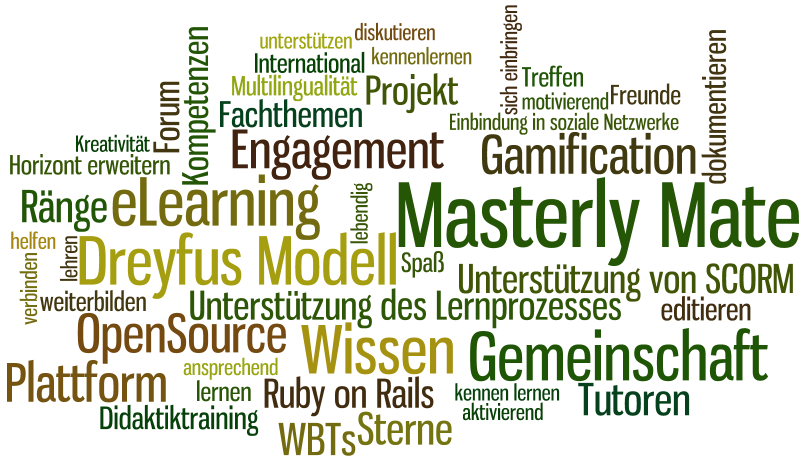
\includegraphics[width=1\textwidth]{MasterlyMateWolke.png}
\caption{Wortwolke über die "`Masterly Mate"'-Idee}\label{ref:wolkeMM}
\end{figure}

Das Projekt nimmt sich eine Art Lernplattform zum Ziel, auf der Lernende auf
Lehrende treffen sollen. Dabei entstehen Situationen, in der eine lehrende
Person zu einer lernenden wird, und umgekehrt. Es sollen Diskussionen über
bestimmte Fachgebiete stattfinden können und ideale Tutoren für bestimmte
Fragestellungen gefunden werden. Da es nichts zu gewinnen gibt, engagiert sich
jeder Teilnehmer freiwillig. Er erhält Wissen und kann dieses im nächsten Moment
an weitere interessierte Personen weitergeben, was sein eigenes Wissen erneut
festigt. Lehrstunden sollen im gemütlichen Umfeld, wie Caffees oder Parks
stattfinden. Masterly Mate bietet dazu eine regionale Suche an, mit deren Hilfe
Lernende und Lehrende aufeinander treffen. Dem Duo steht es auch offen auf
andere Kommunikationskanäle, wie Chat oder E-Mail, zu wechseln. Jeder Nutzer
kann als Tutor für sein Fachgebiet oder seine Fachgebiete fungieren.

Um stets einen idealen Tutor zu finden, folgt die Idee dem Dreyfus fünf Etappen
Modell mentaler Aktivitäten, welches in Abschnitt \ref{ref:dreyfus} näher
beschrieben wird. So ist gewährleistet, dass ein Neuling die Inhalte von einer
Person erklärt bekommt, die selbst noch im Lernprozess steckt und es können
Inhalte, Tipps und Hinweise auf passendem Niveau ausgetauscht werden.

Letztlich soll das Ziel der Mitgliedschaft auf der Plattform nicht sein, der
beste Guru eines Faches zu werden oder der beste Lehrer zu werden. Es geht darum
Teil einer Bildungsgemeinschaft zu sein und sich gegenseitig engagiert zu
unterstützen.

\section{Motivation und Notwendigkeit}\label{ref:projectMotivation}
Die Motivation zu dieser Idee entstand aus der interessanten und
erwartungsvollen Kombination von eLearning und Gamification. Hinzu kommt die
heute populäre Vorstellung von Blended Learning, wodurch das doch sehr trockene
und eintönige Durcharbeiten von WBTs durch Lehreinheiten mit einem Tutor
unterstützt wird.

Masterly Mate soll eine zentrale Anlaufstelle für diverse Weiterbildungs- und
Lernangelegenheiten sein. Unabhängig davon, ob die Motivation privatem Interesse
oder dem eigenen Bildungsweg entspringt, soll jeder Interessent wissen, dass
die Plattform Antworten bietet.

Die Notwendigkeit resultiert aus der fehlenden Fähigkeit des Internets,
Sachverhalte erläutern zu können. Heute ist es Usus beim Recherchieren das
Internet zu gebrauchen, in dem rohe Daten und Informationen vorliegen. Wissen
ist dort eher rar. Es gibt bisher nur wenige Plattformen, wie Wikipedia, die
existieren, um Wissen zu publizieren, jedoch fehlt auch dort eine erklärende und
erläuternde Komponente durch einen Menschen. Dieses Manko soll Masterly Mate
ausgleichen.

\section{Abgrenzung}
Das Projektergebnis behauptet keinen Anspruch auf ein vollwertiges \ac{LMS}. Es
fehlt die Komponente zur Organisation kompletter Lernpakete. In Masterly Mate
stehen die WBTs unabhängig da. Sie sind allein Mittel zum Zweck als Beleg für
die fachliche Kompetenz.

Weiterhin soll es Wikipedia nicht ersetzen. Das Projektergebnis bietet keine
ausformulierten Texte oder Artikel zu Lerninhalten. Der Fokus liegt wesentlich
stärker auf der Komponente Wissen zu vermitteln.

\section{Zielsetzung}
Da das Projekt insgesamt auf einen längeren Zeitraum angesetzt ist, lässt es
sich nicht innerhalb der Bearbeitungszeit der vorliegenden Studienarbeit
umsetzen. Aus diesem Grund sind die Ziele zum einen in operative und zum anderen
in strategische zu unterteilen. 

\subsection{Operative Ziele}
Wie in Kapitel \ref{ref:chaptIntroduction} bereits angerissen wurde, soll zu
Projektende ein funktionaler Prototyp stehen. Auch ist ein Konzept angedacht,
welches der Bekanntmachung von Masterly Mate dient. Eventuell wird sich bis
dahin eine kleine, lebendige Gemeinschaft gebildet haben, die die Plattform
nutzt und um Inhalte erweitert. Die ersten Nutzer sollen automatisch unabhängig
ihres didaktischen Grades\footnote{näher erläutert in Abschnitt
\ref{ref:rankTeach}} Autoren sein. So ist gewährleistet, dass Inhalte für neue
Nutzer bereits existieren. 

Das Projekt als Ganzes soll einen leichten Start haben. Sind die Ziele für die
ersten Nutzer zu hoch gesteckt, resultiert aus der geringen Anzahl von Nutzern
und der damit schwer erreichbaren nächsten Rängen Frustration und Unwille zur
Nutzung der Plattform. Somit ist angedacht, die erforderliche Punktzahl für
höhere Ränge (siehe Abschinitt \ref{ref:dreyfus}) mit der Menge der Nutzer zu
skalieren.

\subsection{Strategische Ziele}
Längerfristig betrachtet soll eine rege und große Gemeinschaft entstehen, die
Hilfsbereitschaft nicht scheut. Dazu wird bereits zu Beginn der Entwicklung eine
Internationalisierung\footnote{siehe Abschnitt \ref{ref:internationalisierung}}
berücksichtigt. Masterly Mate soll zur, in Abschnitt \ref{ref:projectMotivation}
beschriebenen, zentralen Anlaufstelle heranwachsen.

Dabei werden, um den Reiz am Lernen zu erhöhen, mit der Menge der Nutzer die
Anforderungen für die jeweils nächsten Ränge erhöht. Denn je mehr Beteiligung
die Plattform erfährt, desto wahrscheinlicher ist es, einen Tutor in der
jeweiligen Region zu finden. Damit wird es auch immer einfacher, Punkte für den
didaktischen Rang zu sammeln.
	% Da zu erwarten ist, dass nicht das komplette Konzept in dieser Studienarbeit
% realisiert werden kann, erfolgt die Entwicklung und Publikation mit einer
% OpenSource-Lizenz. Um die Weiterentwicklung für eine Community attraktiv zu
% machen, wurde mit Ruby on Rails ein Framework verwendet, welches sich im
% OpenSource-Bereich einer großen Beliebtheit erfreut.

% Meister, also Mitglieder mit bester didaktischer
% Qualifikation, werden Autoren von WBTs. Dadurch soll Qualität 

\chapter{Konzeption der Plattform}\label{ref:chaptConcept}
Ziel des Systems ist die Vermittlung von Lerninhalten in einer sich gegenseitig
Unterstützenden Gemeinschaft. Zu diesem Zweck folgt das Konzept einer Mischung
aus Lern- und Datingplattform -- es werden Lerninhalte bereitgestellt, zu denen
Tutoren vermittelt werden.

\section{Namensgebung}
Der Name "`Masterly Mate"' entstand aus dem höchsten Rang im Dreyfus-Modell
(siehe Abschnitt \ref{ref:dreyfus}) und einem beliebten Getränk im
Informatikerkreis, beziehungsweise dem englischen Begriff für Kumpel/Kamerad.

So lässt sich der Name frei als meisterlicher Kamerad übersetzen, was die
erwünschte offene und freundliche Kommunikation auf der Plattform ausdrücken
soll.

\section{Das Dreyfus-Modell mentaler Aktivitäten}\label{ref:dreyfus}
Inhalt des Dreyfus-Modells ist das Hinterfragen, welche Person einer anderen
einen bestimmten Sachverhalt erklären sollte. Dabei wird insbesondere
berücksichtigt, wie groß der Unterschied der Fachkompetenz zwischen Lernenden
und Lehrenden ist. Dazu wurden insgesamt fünf Ränge\footnote{Novice, Competence,
Proficiency, Expertise, Mastery} definiert. 

Allgemein formuliert sollte kein Experte einem Neuling etwas erklären. Steigt
man neu in ein Fachgebiet ein, so sind zunächst simple und einfache Beispiele
verbunden mit einem engen Betrachtungswinkel des Sachverhalts sehr hilfreich.
Ein Experte würde den Neuling mit unnötigen Details überhäufen. Weitere
detailliertere Erklärungen zu den Rängen finden sich in \cite{gruben:2012}.

Für das Produkt der vorliegenden Studienarbeit wird das Modell angepasst. So
ergeben sich vier fachliche Ränge. Hinzu kommen Ränge für Tutoren, welche einem
Nutzer den fünften Rang nach dem Dreyfus-Modell erreichen lässt. Hinzu kommt,
dass der fachliche Rang regelmäßig vom Nutzer bestätigt werden muss. Nach einem
Jahr im selben Rang wird der Nutzer aufgefordert einen Test zu absolvieren.
Besteht er den Test nicht, oder ignoriert er diesen, so fällt der Nutzer
automatisch um einen Rang. Da es keinen Rang unterhalb von "`novice"' gibt,
werden Nutzer automatisch gelöscht, die den Test für den untersten Rang nicht
bestehen. Diese Vorgehensweise wird so umgesetzt, da davon ausgegangen werden
kann, dass ein aktiver Nutzer innerhalb eines Jahres den nächst höheren Rang
erreicht. Weiterhin werden so inaktive und nicht interessierte Nutzer
automatisch entfernt, was in einer regen Gemeinschaft resultiert. Dem Problem
von Accounts, hinter dem kein aktiver Nutzer\footnote{sogenannten Zombies} mehr
steht, wird somit vorgebeugt. 

\subsection{Fachlicher Rang}\label{ref:rankTopic}
Mit dem Durcharbeiten von WBTs kann ein Nutzer im fachlichen Rang aufsteigen.
Der Hintergrund ist, dass er mit korrekten Antworten im Prüfungsteil der WBTs
seine fachliche Kompetenz unter Beweis stellt. Demgegenüber werden bei falschen
Antworten im Quiz keine negativen Punkte angerechtnet. Je nachdem, wie gut ein
Test ausfällt, erhält er eine bestimmte Anzahl an Punkten. Abhängig vom Grad des
aktuellen fachlichen Rangs wird auch die notwendige Punktzahl für den nächsten
Rang erhöht. Der Aufbau folgt also analog einer Exponentialfunktion. Wie in
Abbildung \ref{ref:vertPunkt} zu sehen ist, benötigt man im Vergleich mit den
didaktischen Rängen im fachlichen Level mehr Punkte für den nächsten Rang. Im
Gegensatz dazu wird hier maximal der Experten-Rang erreicht. In der Abbildung
ist der Rang des Experten nicht zu sehen, da dieser das Erreichen der
notwendigen kompletten Punktzahl symbolisiert.

Selbstverständlich können weitere WBTs durchgearbeitet werden, diese bessern
jedoch nicht das Punktekonto für den fachlichen Rang auf. Dem Anwender ist
freigestellt, ob er sich nun, wo er Experte in einem Fachgebiet ist, einem
anderen Wissensgebiet widmet, um dort als Neuling von Vorn anzufangen.

\subsection{Ränge für Tutoren}\label{ref:rankTeach}
Als Tutor wird man von den Lernenden beurteilt, die man in einem gewissen
Fachgebiet unterstützt hat. Im Gegensatz zu den fachlichen Rängen sind die
didaktischen Ränge vom Fach unabhängig. Auch bleiben sie über alle fachlichen
Ränge hinweg erhalten. Ein weiterer Unterschied ist, dass man als Tutor nicht
Punkte, sondern Sterne sammelt. Jede gute Bewertung (daumen rauf) gibt einen
Schritt in Richtung weiteren Stern. Eine schlechte Bewertung (daumen runter)
stellt dazu einen direkten Gegensatz dar. Beide Bewertungsrichtungen verhalten
sich ausgeglichen und es kristallisieren sich Tutoren heraus, die fachliche
Inhalte für jedermann verständlich zu erklären wissen. So ist auch
gewährleistet, dass sich meisterliche Tutoren nicht auf ihren vier Sternen
"`ausruhen"'. 

Meisterliche Tutoren verfügen auch über das Privileg eigene WBTs in die
Plattform einbringen zu können. Den niederen Rängen ist dies verwehrt, da diese
unter Umständen Sachverhalte nicht allgemeinverständlich zu erläutern wissen.
Auch sind meisterliche Tutoren dazu privilegiert sämtliche fachliche Ränge
unterrichten zu können, während für gewöhnlich Lernende nur von Tutoren
unterwiesen werden, die maximal zwei fachliche Ränge über ihnen stehen.

Gegenüber den fachlichen Rängen ist in Abbildung \ref{ref:vertPunkt} zu sehen,
dass für den nächsten Rang bzw. Stern vergleichsweise weniger Punkte zu
erreichen sind. Demgegenüber lässt sich nur als Tutor der Rang des Meisters, der
vier Sternen entspricht, erreichen. Dieser Rang ist in der Abbildung nicht zu
sehen, da er analog zum fachlichen Rang den Erhalt aller möglichen Punkte
symbolisiert. Ein Meister hat durch das Erhalten der höchsten Wertung für die
didaktische Fähigkeit bereits bewiesen, dass er Spaß an der Vermittlung von
Wissen hat. Demnach bedarf er keiner weiteren Motivation eines höheren Ranges.
Vielmehr möchte er keine negativen Bewertungen seiner Lernenden erhalten und
bemüht sich der weiteren hochwertigen Qualität seiner Lerneinheiten.

\begin{figure}[H]
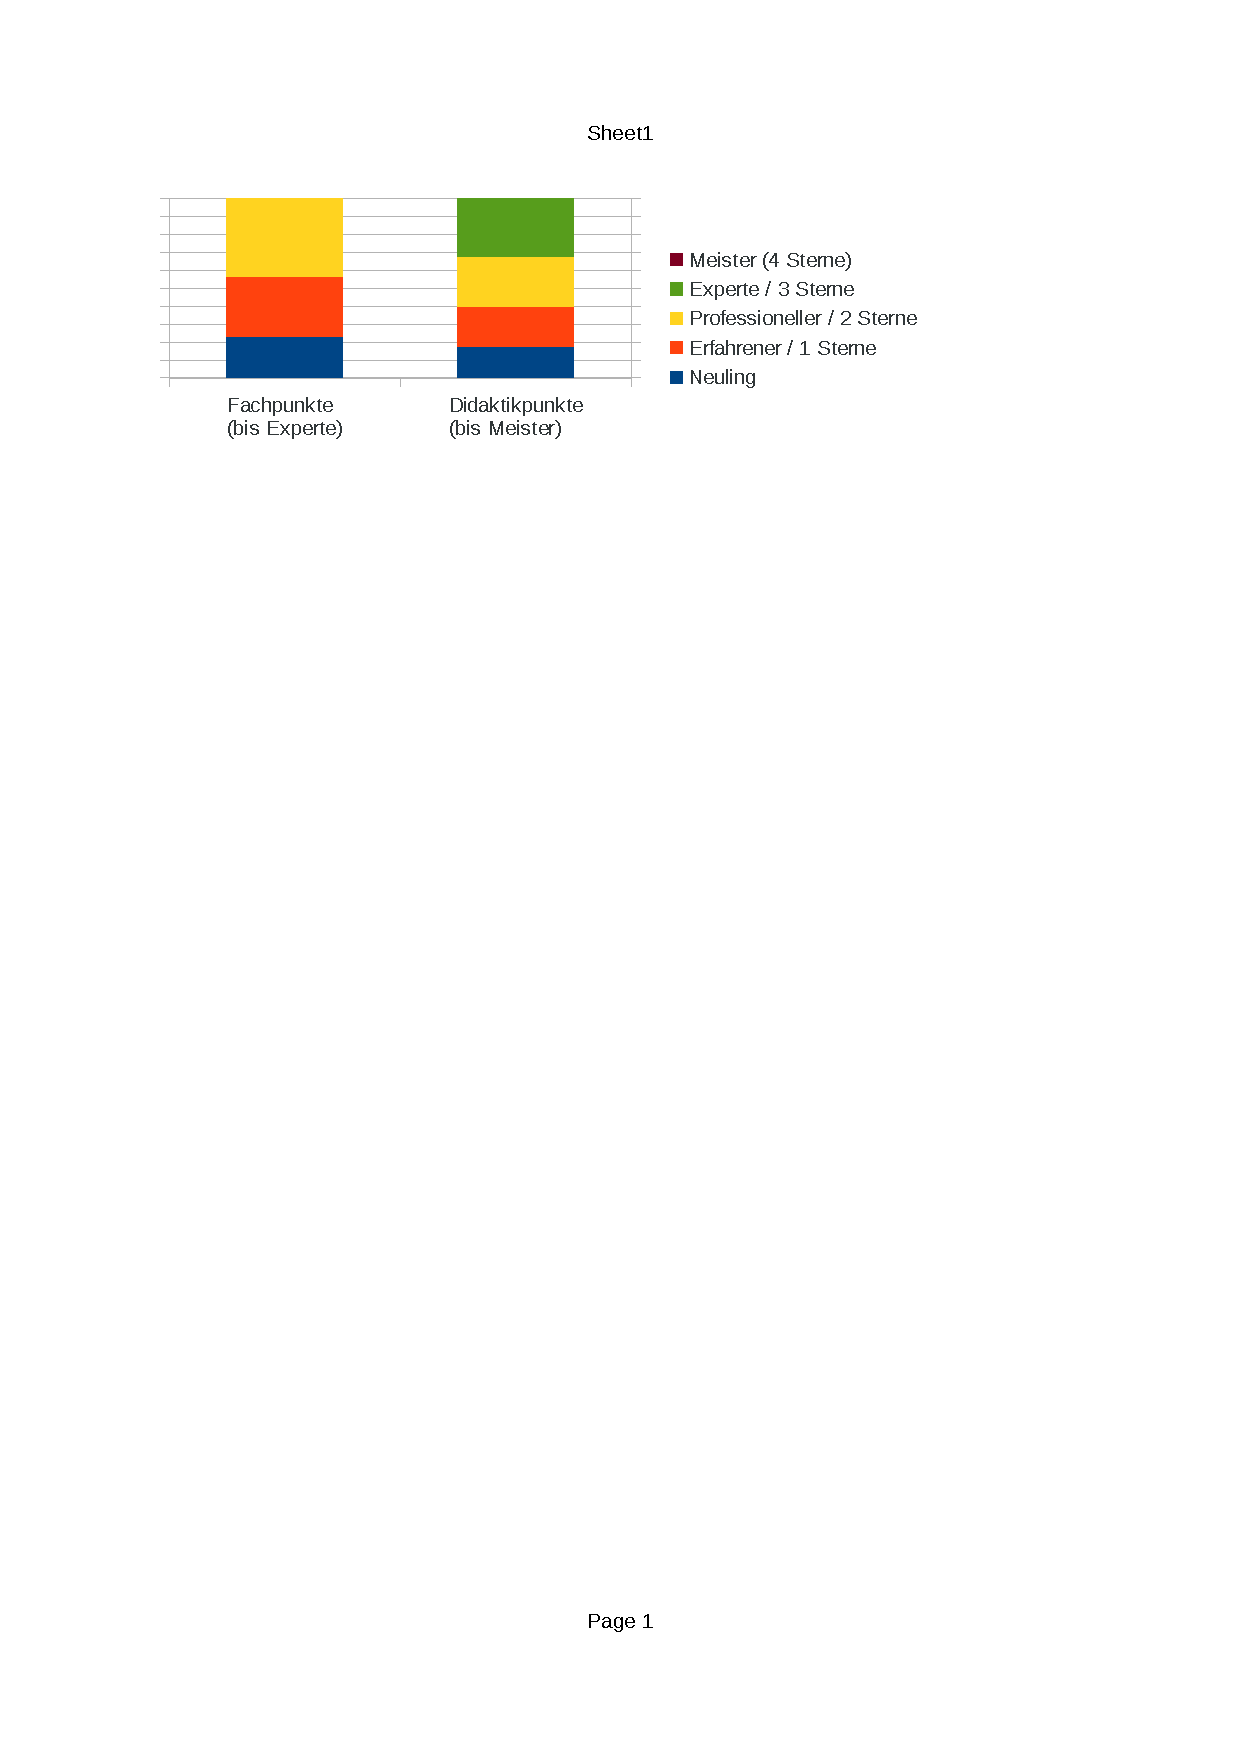
\includegraphics[width=1\textwidth]{verteilungDerPunkte.png}
\caption{Verteilung der Punkte}\label{ref:vertPunkt}
\end{figure}

\section{Rollen für Anwender}
Passend zum zuvor beschriebenen Konzept werden drei Rollen für Anwender
definiert. Dabei ist das Innehaben mehrerer Rollen zur gleichen Zeit ein Teil
des Modells. Zusammenfassend sind die Rechte und Pflichten eines Nutzers in den
verschieden Rollen in Tabelle \ref{tab:privilegesRoles} am Ende des
Kapitels aufgeführt.

\subsection{Administrator}
Der Administrator ist der Verwalter der Plattform und damit für den
reibungslosen Ablauf seitens der Nutzer verantwortlich. Dazu kontrolliert er den
Zusammenhalt des Systems und greift bei inkonsistenzen oder Fehlern ein. Auch
bildet er die Schnittstelle zur Community, die sich in der Weiterentwicklung von
Masterly Mate engagiert.

\subsection{Lernender}
Der Lernende bildet die Hauptzielgruppe des Systems. Er soll WBTs finden, diese
durcharbeiten können und sich an Tutoren wenden, falls er auf ein Problem oder
Unklarheiten stößt. Dazu bietet Masterly Mate ihm das auffinden eines an sein
Fachwissen angepasstes Training. Weiterhin kann er Tutoren kontaktieren, die in
seinem Umkreis wohnen und passend zu seinem Rang Inhalte zu erläutern verstehen.
Die Lokation wird anhand der Postleitzahl festgemacht.

Ein Lernender kann in seinem fachlichen Level bis zum Experten aufsteigen.
Nähere Erläuterungen zu den fachlichen Rängen wurden in Abschnitt
\ref{ref:rankTopic} aufgeführt.

\subsection{Tutor}
Ein Lernender kann ab dem zweiten fachlichen Rang des Dreyfus-Modells (siehe
\ref{ref:dreyfus}) in seinem Profil die Einstellung "`Tutor"' anwählen. Damit
erscheint er unter den Suchergebnissen für Lernende, die einen Tutor suchen. Als
Tutor wird man von Lernenden gefunden, die Unterstützung in einem Fachgebiet
suchen.

\begin{table}[ht] \centering \caption{Rechte und Pflichten der verschiedenen
Rollen}\label{tab:privilegesRoles}
\begin{tabular}{|p{3.2cm}|p{1.7cm}|p{2,5cm}|p{2.7cm}|p{2.5cm}|}\hline
&\textbf{Ad\-mi\-nis\-tra\-tor}&\textbf{Lernender}&\textbf{Lehrender
(Tutor)}&\textbf{meis\-ter\-lich\-er Tutor}\\\hline\hline
 
WBTs lesen&\ding{51}&\ding{51}&\ding{51}&\ding{51}\\\hline
 
Punkte aus Quiz in WBTs ziehen&\ding{55}&\ding{51}
(bis Experte) &\ding{55}&\ding{55}\\\hline

WBTs erstellen \& löschen &\ding{51}&\ding{55}&\ding{55}&\ding{51}
\mbox{(nur eigene)}\\\hline

WBTs bearbeiten &\ding{51}&\ding{55}&\ding{55}&\ding{51}\\\hline\hline

Im Rang steigen &\ding{55}&\ding{51} (bis Experte)&\ding{51}
(bis Meister)&\ding{55}\\\hline

Im Rang fallen &\ding{55}&\ding{51} (bei
nicht bestehen oder ignorieren eines
jährlichen Tests)&\ding{51} (bei zu vielen negativen
Bewertungen)&\ding{51} (bei zu vielen negativen
Bewertungen)\\\hline\hline

Lernende unterweisen&\ding{55}&\ding{55}&\ding{51} (maximal 2
fachliche Ränge unter dem eigenen)&\ding{51} (jeder unterhalb des
eigenen fachlichen Rangs)\\\hline

von Lernenden bewertet
werden&\ding{55}&\ding{55}&\ding{51}&\ding{51}\\\hline\hline

Forum moderieren&\ding{51}&\ding{55}&\ding{55}&\ding{55}\\\hline
zum Forum beitragen&\ding{51}&\ding{51}&\ding{51}&\ding{51}\\\hline
\end{tabular}
\end{table}
	\chapter{Entwurf}\label{ref:chaptScript}
Der in diesem Kapitel beschriebene Entwurf zeigt konkret, wie das Konzept von
Masterly Mate umgesetzt werden wird. Hier werden Schemata und Architekturen
entwickelt, die im Kapitel \ref{ref:chaptImplementation} in Programmcode
umgesetzt werden.

\section{Realisierungsmethodik}
Nachdem in den vorangegangenen Kapiteln das Konzept von Masterly Mate erläutert
wurde, stellt sich die Frage nach einer geeigneten Möglichkeit zur Umsetzung. Da
die Anwendung stets verfügbar, leicht erreichbar, modular und einfach zu
verwalten sein soll, ist \ac{RoR} das Mittel der Wahl. Dieses bietet viele
interessante Features in Form von sogenannten gems, die dank einer regen
Community stets aktualisiert und erweitert werden. Zudem unterstützt es moderne
Programmierparadigmen, wie \ac{DRY} und \ac{KISS}. Dadurch bleibt die Anwendung
aus Sicht der Programmierer übersichtlich und erscheint sehr strukturiert. Das
das Framework der \ac{MVC}-Architektur folgt, schafft einen weiteren Grundstein
zur Trennung von Zuständigkeiten\footnote{bekannter unter "`separation of
concerns"'} und sorgt auch damit für Übersichtlichkeit. 

Weiterhin ist dieses Framework für die Weiterentwicklung im
OpenSource-Bereich prädistiniert, da damit bisher populäre
Webanwendungen, wie Twitter, realisiert wurden.

Darüber hinaus wird darauf geachtet, die Komponenten nach und nach nur dann zu
entwickeln, wenn sie tatsächlich gebraucht werden. Diese Vorgehensweise nach dem
\ac{YAGNI}-Prinzip beugt ein überlaufenes, unübersichtliches und schwer
zu wartendes Produkt vor.

\section{Internationalisierung}\label{ref:internationalisierung}
Die Internationalisierung gewährleistet eine Webanwendung, die möglichst
unabhängig von natürlichen Sprachen ist. Die Internationalisierung wird auch bei
Masterly Mate weitestgehend bereits in der ersten Version eingesetzt.
Die RoR API bietet dafür die Klasse I18n an, mit dessen Hilfe die
Internationalisierung durchgeführt werden kann. Die Bezeichnung I18n
kennzeichnet den Begriff Internationalisierung als Numeronym. Die Zahl 18 steht
für die Anzahl an Buchstaben, die zwischen den Buchstaben I und n liegen.
Die Klasse I18n bietet neben vielen anderen Methoden eine essentielle Methode
an, mit dessen Hilfe die Internationalisierung von Masterly Mate weitestgehend
realisiert werden kann. Die Methode trägt die Bezeichnung t als Kurzform für
translate. Diese Methode erwartet als einzigen Parameter eine Zeichenkette,
welche den Pfad zu dem entsprechenden Sprachstring angibt. Bei der
Initialisierung der RoR Anwendung Masterly Mate, werden sämtliche *.yaml Dateien
aus dem Verzeichnis config/locales/ als Sprachdateien geladen. Der Name einer
Sprachdatei sollte aus Konventionsgründen einer Rails Webanwendung, stets den
Ländercode beinhalten. In der ersten Version von Masterly Mate werden die
Sprachen Deutsch und Englisch unterstützt. Sven Fuchs bietet für sämtliche
Sprachen auf
Github\footnote{\url{https://github.com/svenfuchs/rails-i18n/tree/master/rails/locale}}
vorgefertigte Sprachdateien an. Diese Sprachdateien definieren für die jeweilige
Sprache entsprechende Formatierungen, wie z.B.
Datum- und Zeitangaben. Aber auch die Werte für Labels von
Formularsteuerungskomponenten, wie z.B. die Submit-Schaltfläche, werden in
diesen Sprachdateien festgelegt. Die anwendungsspezifischen Strings müssen
selbstverständlich selbst in *.yaml Sprachdateien definiert und im Verzeichnis
config/locales/ abgelegt werden. Eine RoR Sprachdatei ist hierarchisch
aufgebaut. Die einzelnen Hierarchieebenen werden dann später beim Zugriff auf
ein Sprachstring über ein Punkt voneinander getrennt. Grundlegend definiert man
eine von der natürlichen Sprache unabhängige Zeichenkette dadurch, indem ein
fester Bezeichner gefolgt von einem Doppelpunkt definiert wird. Nach dem
Doppelpunkt folgt die sprachabhängige Zeichenkette. Im Programmcode wird an den
Stellen, an denen eine sprachenunabhängige Zeichenkette ausgegeben werden soll,
die Methode t der Klasse I18n eingesetzt und dieser als Parameter der Pfad zu
dem entsprechenden Bezeichner übergeben.
Masterly Mate ist nahezu vollständig für die Sprachen Deutsch und Englisch
Internationalisiert. Lediglich die von den Nutzern erstellten WBTs sind nicht
Internationalisiert. Einige WBT-Engines bieten den Mechanismus zur
Internationalisierung nicht an. Aus diesem Grund wurde dieses Vorhaben im Rahmen
dieser Studienarbeit vernachlässigt.

\section{Beschreibung des Entwurfsklassendiagramms und
Use-Case}\label{ref:classModel}

\subsection{Use-Case Diagramm}
Im obigen Use-Case Diagramm, sind die einzelnen benötigten Komponenten
enthalten, wie sie die Analyse ergeben hat. Zunächst einmal lassen sich Aktoren
ausmachen, welche in System/Software-Aktoren und menschliche Aktoren aufteilen
lassen. 

Bei den Softwareseitigen Aktoren ergab die Analyse als Aktoren den Webserver,
ein Einzelnes WBT (sie sollen nach Abschluss die Punkte im System eintragen),
das Autorenwerkzeug und den Webbrowser. Auf der Seite der Aktoren ließe sich der
Lernende (Standard-User), Tutor, Autor und Admin ermitteln. Zu beachten ist,
dass die Aufteilung der menschlichen Aktoren auch eine Berechtigungshierarchie
darstellt, wobei ein Lernender die geringsten und ein Admin die meisten
Berechtigungen hat.

Die einzelnen Use Cases werden nun jeweils im folgenden kurz beschrieben. Zu
beachtenn ist dabei noch, dass diese Analyse sich nicht zwingend mit dem
Ergebnis aus der Studienarbeit deckt, da Funktionalitäten auf spätere Releases
verschoben worden sind.

\subsubsection{WBT durcharbeiten} 
Agierende Aktoren: \begin{itemize}
  \item WBT
  \item Lernender
  \item Tutor
  \item Autor
  \item Admin 
\end{itemize}

Ein Benutzer startet ein WBT und schließt es erfolgreich ab bzw.
scheitert oder beendet es vorzeitig. Im Anschluss daran, werden die erreichten
Punkte im System eingetragen. In der Version der Studienarbeit, wird dies noch
vom Benutzer selbst durchgeführt. Später soll dies das WBT übernehmen.
	
\subsubsection{Bewerten}
Agierende Aktoren: \begin{itemize}
  \item Lernender
  \item Tutor
\end{itemize} 

Den Use Case Bewerten gibt es in zwei Ausprägungen. Die erste Ausprägung ist die
Bewertung eines Tutors. Hat ein Lernender oder eine anderer Tutor (im folgenden
beide als "Lernende" bezeichnet) von dem Betreffenden Benutzer Hilfe erhalten,
so kann der Lernende im Anschluss daran diese Hilfe im System bewerten.
Dies kann er mit Sternen und wahlweise mit einem Kommentar tun (Kommentar noch
nicht in der Alpha-Version). Die Zweite Ausprägung ist die Bewertung eines WBTs.
Ein Benutzer muss das WBT dafür abgeschlossen haben. Ebenso wie beim Tutor kann
er dies über Sterne und Kommentare tun.
	
\subsubsection{Sprache verwalen}
Agierende Aktoren: \begin{itemize}
  \item Alle menschlichen Aktoren (Ausprägung Sprache
hinzufügen kann nur der Admin)
\end{itemize}

Ebenso wie im obigen Use Case gibt es hiervon zwei Ausprägungen.
Nummer Eins ist der Use Case Sprache wechseln. Dieser kann von jedem Benutzer
durchgeführt werden und bewirkt, dass alle Zeichenketten in MasterlyMate, welche
in der betreffenden Sprache vorhanden sind, ausgetauscht werden. Use Case Nummer
Zwei kann nur von einem Administrator durchgeführt werden. Und bewirkt die
Erzeugung einer weiteren Sprache, welche eingestellt werden kann. Gegenwärtig
wird dies noch direkt durch eine Änderung der Sprachdateiten getan.

\subsubsection{Profil verwalten}
Agierende Aktoren: \begin{itemize}
  \item Alle menschlichen Aktoren
\end{itemize}

Auch dieser Use Case verfügt über zwei Ausprägungen. Der erste Use Case ist das
bearbeiten eines Profils. Dies kann nur der besitzer des jeweiligen Profils.
Den anderen Use Case kann hingegen jeder Benutzer durchführen. Es handelt sich
dabei um das Betrachten eines Profils. Dies ist insbesondere für die
Kontaktaufnahme eines Benutzers zu einem Tutor notwendig.

\subsubsection{Suchen}
Agierende Aktoren: \begin{itemize}
  \item Alle menschlichen Aktoren
\end{itemize}

Es können sowohl Tutoren als auch WBTs gesucht werden. Dabei wird jeweils
berücksichtigt welches Themengebiet gefragt ist.
	
\subsubsection{Themengebiet abfragen}
Agierende Aktoren: \begin{itemize}
  \item Webserver
\end{itemize}

Der Webserver überprüft bei einer Suchanfrage die einzelnen Themen.
	
\subsubsection{Themen verwalten}
Agierende Aktoren: \begin{itemize}
  \item Admin
  \item Webserver
\end{itemize}

Nur der Admin kann die beiden Ausprägungen dieses Use Cases durchführen, welche
das Hinzufügen und Löschen eines Themas darstellen.
	
\subsubsection{WBT verwalten}
Agierende Aktoren: \begin{itemize}
  \item Admin
  \item Autor
  \item Webserver
\end{itemize}

Dieser Use Case besitzt drei Ausprägungen. Admin und Autor können WBTs
einbinden. Es kann jedoch nur der User, welcher ein WBT eingebunden hat, dieses
auch wieder entfernen bzw. ersetzen. Dies gilt nicht, wenn der betreffende
Benutzer ein Administrator ist. Dieser kann jedes WBT löschen oder ersetzen.
	

\subsection{Entwurfsklassendiagramm}
In dem Entwurfsklassendiagramm, sind die Models und ihre Beziehungen zueinander
dargestellt. Diese Modelle bilden einzelne Konzepte im System ab. So stellt User
ein Zentrales Modell dar, welches als Abbildung eines Benutzers im System für
die Authentifizierung verantwortlich trägt. Außerdem werden dem User
verschiedene Themen und WBTs zugeordnet. Diese Verbindungen benötigen jeweils
Assoziationsklassen. Dies liegt daran, dass es in dieser Verbindung Attribute
gibt, welche sich nicht eindeutig User oder WBT bzw. Thema zuordnen lassen. Bei
der Verbindung User-Thema benötigt man ein Attribut für die Punkte, welche
bisher von dem User in dem System erziehlt worden sind. Außerdem muss klar sein
welchen Rang ein User in dem jeweiligen Thema inne hat. Die Verbindung User-WBT
dagegen benötigt eine Variable um zu hinterlegen ob ein User das WBT bereits
einmal abgeschlossen hat und wenn ja, wie viele Punkte er erreicht hat. Im folgenden
wird auf die Modelle des UML-Diagrammes näher eingegangen. Dazu sei noch
angemerkt, dass zwischen einem realen Konzept und dem des Models underschieden
wird. D.h. wenn z.B. im Folgenden vom User die Rede ist, dann ist hierbei das
Model oder eine Instanz der User-Klasse gemeint. Wird hingegen vom Benutzer
gesprochen, so ist auch tatsächlich jener gemeint.  

\subsubsection{WBT}\label{ref:objectWBT}
Das WBT-Model verfügt über eine ID, sowie über einen Pfad zur eigentliche
SCORM-Datei. Wie bereits erwähnt ist es einem oder mehreren Themen (Topics)
zugeordnet. Auf Datenbankseite bedeutet dies, dass eine Zwischenentität zwischen
Topic und WBT eingeführt werden muss. 

\subsubsection{Topic}
Im UML-Diagramm ist ersichtlich, dass das Model Topic eine referenz auf sich
selbst besitzt. In dieser Referenz kann ein Topic sowohl die Rolle des über- als
auch des Unterthemas bekleiden. Unterthemen dienen einer genaueren Unterteilung
der WBTs. Tobics werden mit ihrem Namen identifiziert. Dies gilt auch für die
übergeordneten Topics. Dies bedeutet, dass ein Unterthema die Information
besitzt, zu welchem Topic es gehört. Diese vorgehensweise ist auch für die
Datenbank hilfreich, da so der Maxime entsprochen wird, den Fremdschlüssel auf
der N-Seite zu notieren.

\subsubsection{User}
Das Dritte große und wahrscheinlich sogar größte Model ist der User. Er ist
gekennzeichnet durch einen Benutzernamen, Vor- und Nachname, Passwort,
Geburtstag und einer Email-Adresse. Der User, stellt die Benutzer im System dar.
Er wird für die Registrierung und Authentifizierung verwendet. Des Weiteren
werden ihm die Punkte zugeordnet, welche ein Registrierter Benutzer in einem WBT
erzielt. Damit werden ebenso die Ränge dem Benutzer zugeordnet, von welchen er
beliebig viele haben kann (siehe dazu Model: Ränge). 
Ein Benutzer ist außerdem in einer oder mehrerer der möglichen Gruppen
eingeordnet.
Über diese wird geregelt, welche berechtigungen er im System hat. Näheres dazu
ist im entsprechenden Abschnitt zu finden.
Eine besondere Funktion fällt der Zuordnung eines User zu einer Location zu. Mit
ihr ist es möglich, dass Benutzer Tutoren in der Nähe ihrer eigenen Wohnstätte
finden können (Auch dazu, sie im entsprechenden Abschnitt).

\subsubsection{Group}
Die Gruppen werden zur Festlegung der Berechtigungen verwendet. Ein User
kann in beliebig vielen Gruppen sein und diese wiederum kann beliebig viele User
enthalten. Die Gruppen im System sind die Administratoren, welche volle Rechte
im System besitzen. Die etwas schwächeren Tutoren können WBT hochladen und ihr
eigenes löschen. Außerdem können sie von anderen Usern bewertet werden. Die
Dritte vorhandene Gruppe sind die normalen User. Diese können lediglich WBTs
durcharbeiten, Profile von anderen Usern einsehen, sowie ihr eigenes bearbeiten.
Implizit vorhanden, jedoch nicht implementiert sein soll die Gäste-Gruppe. Diese
umfasst alle Benutzer, welche keinen User im System besitzen.

\subsubsection{Location}
Eine Location beschreibt den groben Standort an dem ein Benutzer wohnt. Daher
verfügt dieses Model auch nicht über die kompletten Adressdaten eines Benutzers,
sondern nur über die Stadt, die Postleitzahl sowie das Land. Da die Location
einzig den Sinn hat, die Suche nach geeigneten Tutoren einzugrenzen ist eine
genauere Standortsbestimmung nicht notwendig. Da es mehrere User gegen kann, die
der gleich Location zugeordnet sind, ist wird diese auf der User-Seite durch die
entsprechende ID der Location identifiziert. 

\subsubsection{Assessment}
Das Assesment bildet als Assoziationsklasse zwischen User und Topic die
Beziehung zwischen dem User und einem Topic ab. In ihr wird gespeichert, wie
viele Punkte er durch die Absolvierung von WBTs in einem Thema erreicht hat.
Entsprechend zeigt das Assesment auch den Rang an, den ein Benutzer in einem
bestimmten Thema erreicht hat.

\subsubsection{Rank}
Der Rang eines Benutzer spiegelt den Erfahrungsstand wieder, den ein Benutzer in
einem Thema erreicht hat. Er wird bei entsprechender Punktzahl (Erspielte Punkte
bzw. Sterne) vom System vergeben.

\section{Funktionalitäten aus Nutzersicht}
Prinzipiell ist Masterly Mate aus zwei Komplexen aufgebaut. Zum einen kann sich
ein Nutzer fachlich weiterbilden. Zum Anderen bietet ein Nutzer als Tutor seine
Hilfe für ein bestimmtes Fachgebiet an.

\subsection{Masterly Mate für Lernende}
Aus Sicht der Lernenden baut sich Masterly Mate aus den folgenden Komponenten
auf.

\subsubsection{Registrieren und Einloggen}
Ein neuer Nutzer wird sich zunächst registrieren. Ist dies bereits geschehen,
kann er sich einloggen und sich dem Bearbeiten von WBTs oder der Administration
seines Profils widmen.

\subsubsection{Durcharbeiten von WBTs}
Ist ein Nutzer an Weiterbildungsangeboten interessiert, so geht er ein oder
mehrere WBTs durch. Dazu erhält er nach einer passenden Filterung der Ergebnisse
anhand einer Themenwahl und des dazugehörigen fachlichen Ranges (siehe Abschnitt
\ref{ref:autoResult}) eine verfügbare Liste an WBTs, die er nach seinem Gusto
bearbeiten kann.

\subsubsection{Tutorensuche}
Stößt der Lernende beim Durcharbeiten von WBTs auf ein fachliches Problem, so
kann er einen Tutor aufsuchen. Die Darbietung passender Tutoren erfolgt ebenso
nach einer automatischen Filterung. Die Filterung wird auch hier anhand des
fachlichen Rangs des Lernenden und des Themengebiets vorgenommen. Hinzu kommt
der didaktische Rang des Tutoren und die jeweils angegebene Postleitzahl
Lernenden und des Tutors, sodass ein Treffen aufgrund der räumlichen Nähe
einfacher möglicht wird.

\subsubsection{Profil administrieren}
Jedem Nutzer ist es erlaubt, sein eigenes Profil zu administrieren. Dort kann er
sein Profilbild und andere persönliche Angaben, wie Spitzname, Name und
Postleitzahl ändern. Zusätzlich kann er hier eine Option anhaken, die ihm zum
Tutor macht. Damit erscheint er für andere Lernende in den Suchergebnissen für
passende Tutoren. Demgegenüber kann er den Haken wieder entfernen, falls er kein
Tutor mehr sein möchte.

\subsubsection{Navigation, Impressum, Kontakt}
Eine übersichtliche und nicht zu detailierte Navigation für Masterly Mate war
ebenfalls ein Ziel dieser Studienarbeit. Die Funktionsweise eines
Navigationsmoduls sollte nicht neu entwickelt werden. Aus diesem Grund wurden
einige vorgefertigte Gems für die Navigation in Betracht gezogen. Das Gem,
welches letztlich für die Navigation in Masterly Mate eingesetzt wurde, nennt
sich Simple-Navigation\footnote{\url{https://github.com/andi/simple-navigation}}.
Die Handhabung dieses Gems ist sehr einfach und darüber hinaus bietet es eine
übersichtliche Infrastruktur und somit ein Grundkonzept für die Funktionsweise
einer Navigation. Die Elemente der Navigationsleiste werden an einer zentralen
Stelle in der config/navigation.rb definiert. Auch das Festlegen von
Subelementen ist möglich. Weiterhin kann man eine von mehreren 
Darstellungsarten, wie z.B. einer ungeordneten HTML Liste, Linklisten,
Breadcrumbs, etc. für das Navigationsmoduls auswählen. Für Masterly Mate wird
eine entsprechend mit CSS formatierte Linkliste eingesetzt.
Für das Impressum wurde im Rahmen dieser Studienarbeit keine eigene Seite in der
Webanwendung vorgesehen. Dieses befindet sich daher in der Fußleiste von
Masterly Mate. Auch ein Kontaktformular wurde in dieser Arbeit nicht vorgesehen.
Der Kontakt erfolgt in der aktuellen Version über das Anschreiben an die
Entwickler von Masterly Mate per E-Mail. 

\subsubsection{Themen}
Themen fungieren für den Benutzer zum Einen als Suchfilter bei der Suche nach
den WBTs. Dies sorgt dafür, dass der Benutzer ohne umschweife auf WBTs zugreifen
kann, welche für ihn interessant sind. Außerdem dienen Themen dazu, die
unterschiedlichen Ränge, welche ein Benutzer zur selben Zeit in Masterly Mate
haben kann, voneinanderabzugrenzen. Jeder Benutzer kann in einem Thema nur genau
einen Rang inne haben. Umgekehrt kann er jedoch in beliebig vielen Themen einen
Rang haben.

Zu diskutieren ist, hierbei ob ein Benutzer jeweils in einzelnen Unterthemen
einen Rang inne hat und auch im Oberthema oder nicht. Wenn er in jedem wirklich
Thema einen Rang inne haben kann ist außerdem zu klären, wie sich das auf den
Rang im Überthema auswirkt. Er könnte in diesem Falle sowohl die erzielten
Punkte gutgeschrieben bekommen als auch in allen darüberliegenden Themen. Dann
hätte er in dem Überthema einen Rang, welcher mindestens so hoch ist, wie der
höchste Rang in einem der Unterthemen. 
In einem anderen Falle, namentlich Ränge in allen Themen ohne das kaskadieren
der Punkte, wäre es möglich, dass der Benutzer in einem Unterthema Meister sein
könnte im Übergeordneten jedoch nur Erfahrener, da er in dem Überthema nur die
Punkte erhält, welche direkt diesem Thema untergeordnet sind.
Ein ganz anderer Fall hingegen wäre es, wenn der Benutzer nur in einem der
Überthemen einen Rang haben könnte und die Unterthemen einzig und allein der
Unterteilung dienen. In diesem Falle müsste man im Datensatz nachprüfen ob das
Thema, zu dem das abgeschlossene WBT gehört, ein übergeordnetes Thema hat. Ist
dies der Fall so müssten dieses Thema überprüft werden. Dieser Vorgang müsste
solange fortgesetzt werden, bis das hierarchisch höchste Thema gefunden ist.
In diesem Thema würden dann die Punkte dem Benutzer zugeteilt.

Ein ganz anderes Problem stellt das löschen von Themen dar. Auch hier gibt es
mehrere Möglichkeiten. So ist es denkbar, dass bei einer Löschung eines Themas,
alle Unterthemen mit WBTs gelöscht werden. Dies sollte allerdings mit Vorsicht
genossen werden und am besten mit einer oder eventuell zwei Abfragen hinterfragt
und bestätigt werden.
Eine andere, weniger gefährliche Option wäre es, die enthaltenen Unterthemen und
WBTs dem übergeordneten Thema des gelöschten Themas zuzuordnen. In diesem Fall
ist es notwendig ein Root-Thema zu definieren, welches alle Themen beinhaltet.
In diesem Falle könnte es allerdings Themen geben, die nur in dem Root-Thema
enthalten sind. D.h. es müsste möglich sein in diesem Thema einen Rang
zu erhalten (Man könnte sich an dieser Stelle fragen ob es nicht Sinvoll wäre,
dort ein WBT zur "`frage nach dem Leben, dem Universum und Allem"' zu
platzieren, weiter sei die Frage erlaubt, ob ein Meister in diesem Thema sich
``Master of the Universe'' zu nennen habe). Alternativ könnte man abfragen ob
ein WBT sich nur innerhalb des Root-Themas befindet und wenn dies der Fall ist,
dem Benutzer den Zugriff verwehren.  

\subsection{Masterly Mate aus Sicht eines Tutors}
Ein Tutor ist quasi eine erweiterte Form eines Lernenden. So bleiben dem Tutor
die verfügbaren Möglichkeiten eines Lernenden erhalten. Hinzu kommen zwei
weitere Funktionen.

\subsubsection{Lernende unterstützen}
Lernende werden gelegentlich an ihre Grenzen stoßen und Tutoren zu Rate ziehen.
Als Tutor auf Masterly Mate ist man, da man sich selbst in beliebigen
Fachgebieten weiterbilden kann, mit einem Lernenden nahezu gleichgestellt. Dem
Lernenden wir damit eine Hilfe gebende Person auf Augenhöhe vermittelt. 

Im Konzept von Masterly Mate ist nur eine Hilfe der beschriebenen Art
berücksichtigt. Tutoren können sich jedoch darüber hinaus auch auf eine
beliebige andere Art an Lernende wenden, wie zum Beispiel das geben von
Workshops oder halten von Präsentationen.

\subsubsection{WBTs verbessern und hinzufügen}
Hat ein Tutor den Rang des Meisters erreicht, so ist es ihm aufgrund seiner
herausragenden didaktischen Leistungen erlaubt, bestehende WBTs zu verbessern
oder neue zu entwickeln und auf die Plattform zu laden.
	\chapter{Implementierung}\label{ref:chaptImplementation}
\section{Nutzerverwaltung}
\section{Lokationen}
\section{Suche}
\section{SCORM}

	\chapter{Zusammenfassung der Ergebnisse}\label{ref:chaptConclusion}
\begin{k}
\begin{itemize}
  \item Rails unheimlich mächtig, wir sind sehr begeistert
  \item schwierig wird es bei speziellen Dingen, die dann in Ruby programmiert
  werden müssen
\end{itemize}
\end{k}
	\chapter{Fazit und Ausblick}\label{ref:chaptSummary}

\section{Ideen für weitere Versionen}\label{ref:weitereIdeen}
\begin{k}
\begin{itemize}
  \item Nutzer kann eine Liste aller WBTs sehen, die er absolviert hat
  \item Forum
  \item Durchführung von Refactorings für DRY KISS
  \item Profilbild
  \item SCORM RTE implementieren
  \item Mailerfunktionalität
  \item Investierte Zeit mit in das Konzept für Belohnungen einbringen
  \item Am Ende jedes WBT eine Wertung abgeben (zu schwer/zu leicht) -> tendiert
  eine Wertung zu stark in eine Richtung, wird das WBT dem am nächsten passenden
  Rang zugeordnet
\end{itemize}

\subsection{Gamification für Newbies}
\begin{itemize}
    \item Quick-Start Guide (Video-)Instruction, (Video-)Tutorial
    \item Statistical evaluation (Ranking)
    \item Unlock big equipments for the selected design
    \item Possibility of using a Open-ID
    \item Newsletter-Feature
    \item Self-assessment regarding to school grades
  \end{itemize}
  
 \subsection{Gamification für Regulars}
 \begin{itemize}
    \item Collections of Achievements according to the current progression
  \end{itemize}
  
 \subsection{Gamification für Enthusiasten}
 \begin{itemize}
    \item Levels
    \item Dynamic difficulty / i.e. riddles
  \end{itemize}
  
 \subsection{Weitere Möglichkeiten für Gamification}
\begin{itemize}
\item Design Selection (Tamagochi, Avatar)
  \item Assistance possible
  \item Progress bar
  \item status message
  \item discussion room
  \item class room
  \end{itemize}
  
wie schaut das Gamification-Konzept von MM aus? Irgendwie ist Fortschrittsbalken
und Statistik und Möglichkeit als Tutor zu gering bis Meister. Gut ist der
Anreiz, ab Meister WBTs einbringen und editieren zu können. Wie war das mit dem
Avatar oder der UI, die immer besser gestaltet werden kann?

\end{k}

\section{Anschließende Vorhaben}
\begin{k}
sehen, was wird
\begin{itemize}
  \item wirklich nur in Ausnahmefällen eine DE? (siehe
  \ref{ref:blendedLearning})
  \item (un)populär
  \item neue Verwendungszwecke
  \item nur eine Installation oder mehrere
\end{itemize}

kann mithilfe von Masterly Mate ein idealer Lehrer gefunden werden?
\end{k}
	
	% Anhang
	\clearpage
	\pagenumbering{roman}

	% Abbildungsverzeichnis
	\cleardoublepage
	\phantomsection \label{listoffig}
	\addcontentsline{toc}{chapter}{Abbildungsverzeichnis}
	\listoffigures

	%Tabellenverzeichnis
	\cleardoublepage
	\phantomsection \label{listoftab}
	\addcontentsline{toc}{chapter}{Tabellenverzeichnis}
	\listoftables

	% Quellcodeverzeichnis
	\cleardoublepage
	\phantomsection \label{listoflist}
	\addcontentsline{toc}{chapter}{Listings}
	\lstlistoflistings

	% Literaturverzeichnis
	\cleardoublepage
	\phantomsection \label{listoflit}
	\addcontentsline{toc}{chapter}{Literaturverzeichnis}
	\bibliographystyle{agsm}
	\bibliography{studArb2Bib}
\end{document}